\documentclass[border=10pt]{standalone}
\usepackage{tikz}
\usetikzlibrary{shapes,arrows,positioning,decorations.pathreplacing,shadows}

\begin{document}

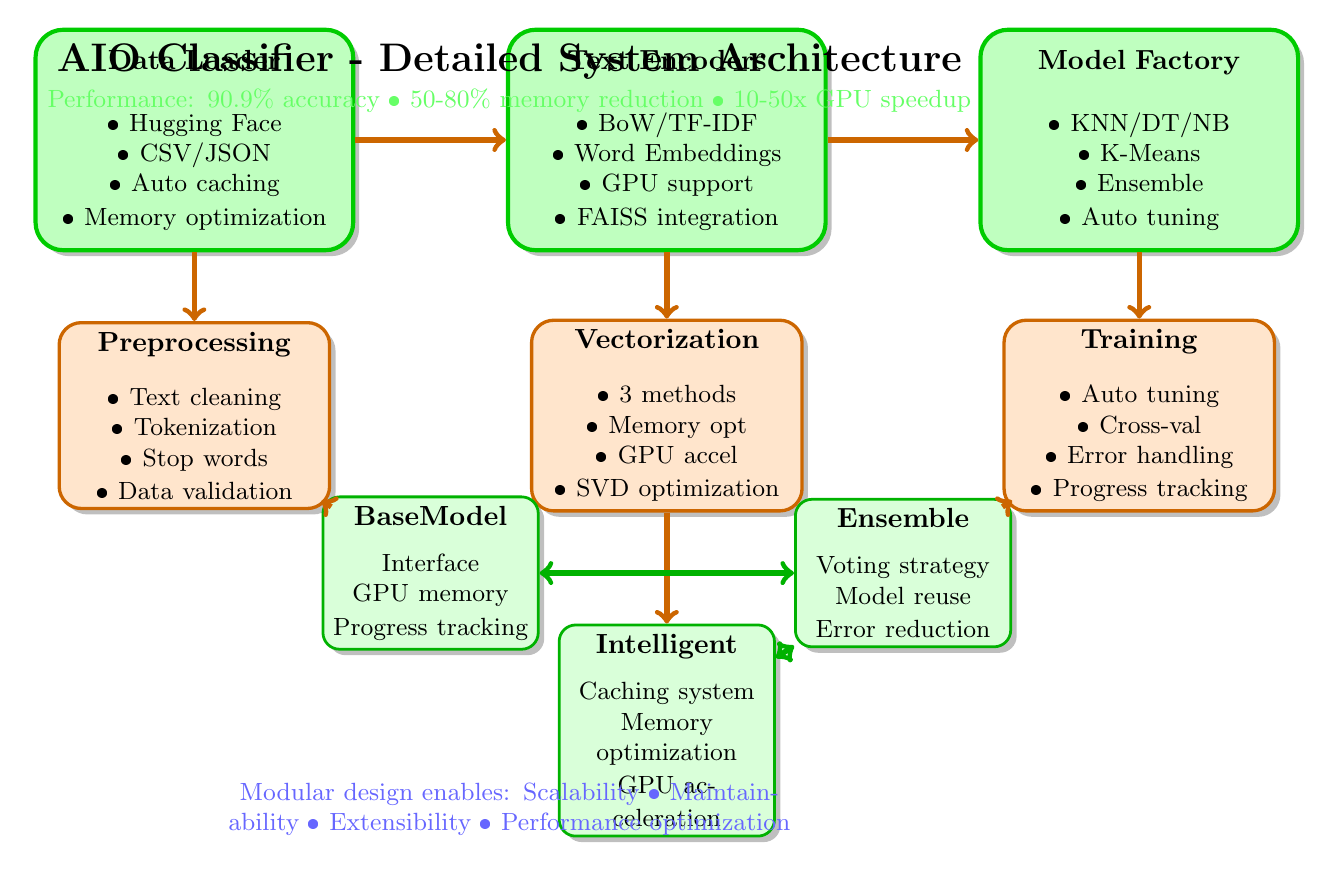
\begin{tikzpicture}[
    % Define styles
    main_component/.style={
        rectangle,
        draw=green!80!black,
        fill=green!25,
        text width=3.8cm,
        text centered,
        minimum height=2.8cm,
        rounded corners=10pt,
        drop shadow,
        line width=1.5pt
    },
    sub_component/.style={
        rectangle,
        draw=orange!80!black,
        fill=orange!20,
        text width=3.2cm,
        text centered,
        minimum height=2.2cm,
        rounded corners=8pt,
        drop shadow,
        line width=1.2pt
    },
    feature_box/.style={
        rectangle,
        draw=green!70!black,
        fill=green!15,
        text width=2.5cm,
        text centered,
        minimum height=1.5cm,
        rounded corners=6pt,
        drop shadow,
        line width=1pt
    },
    arrow/.style={
        ->,
        thick,
        orange!80!black,
        line width=2pt
    },
    double_arrow/.style={
        <->,
        thick,
        green!70!black,
        line width=2pt
    }
]

% Main components
\node[main_component] (data_loader) at (0,6) {
    \textbf{Data Loader}\\[0.4cm]
    \small
    • Hugging Face\\
    • CSV/JSON\\
    • Auto caching\\
    • Memory optimization
};

\node[main_component] (text_encoders) at (6,6) {
    \textbf{Text Encoders}\\[0.4cm]
    \small
    • BoW/TF-IDF\\
    • Word Embeddings\\
    • GPU support\\
    • FAISS integration
};

\node[main_component] (model_factory) at (12,6) {
    \textbf{Model Factory}\\[0.4cm]
    \small
    • KNN/DT/NB\\
    • K-Means\\
    • Ensemble\\
    • Auto tuning
};

% Sub-components
\node[sub_component] (preprocessing) at (0,2.5) {
    \textbf{Preprocessing}\\[0.3cm]
    \small
    • Text cleaning\\
    • Tokenization\\
    • Stop words\\
    • Data validation
};

\node[sub_component] (vectorization) at (6,2.5) {
    \textbf{Vectorization}\\[0.3cm]
    \small
    • 3 methods\\
    • Memory opt\\
    • GPU accel\\
    • SVD optimization
};

\node[sub_component] (training) at (12,2.5) {
    \textbf{Training}\\[0.3cm]
    \small
    • Auto tuning\\
    • Cross-val\\
    • Error handling\\
    • Progress tracking
};

% Feature boxes
\node[feature_box] (base_model) at (3,0.5) {
    \textbf{BaseModel}\\[0.2cm]
    \small
    Interface\\
    GPU memory\\
    Progress tracking
};

\node[feature_box] (ensemble) at (9,0.5) {
    \textbf{Ensemble}\\[0.2cm]
    \small
    Voting strategy\\
    Model reuse\\
    Error reduction
};

\node[feature_box] (caching) at (6,-1.5) {
    \textbf{Intelligent}\\[0.2cm]
    \small
    Caching system\\
    Memory optimization\\
    GPU acceleration
};

% Main flow arrows
\draw[arrow] (data_loader) -- (text_encoders);
\draw[arrow] (text_encoders) -- (model_factory);

% Vertical flow arrows
\draw[arrow] (data_loader) -- (preprocessing);
\draw[arrow] (text_encoders) -- (vectorization);
\draw[arrow] (model_factory) -- (training);

% Feature connections
\draw[arrow] (preprocessing) -- (base_model);
\draw[arrow] (training) -- (ensemble);
\draw[arrow] (vectorization) -- (caching);

% Bidirectional arrows for integration
\draw[double_arrow] (base_model) -- (ensemble);
\draw[double_arrow] (ensemble) -- (caching);

% Add title
\node[font=\Large\bfseries, text width=12cm, text centered] at (4,7) {
    AIO Classifier - Detailed System Architecture
};

% Add performance indicators
\node[font=\small, text width=12cm, text centered, green!60] at (4,6.5) {
    Performance: 90.9\% accuracy • 50-80\% memory reduction • 10-50x GPU speedup
};

% Add flow description
\node[font=\small, text width=12cm, text centered, blue!60] at (4,-2.5) {
    Modular design enables: Scalability • Maintainability • Extensibility • Performance optimization
};

\end{tikzpicture}

\end{document}
